% !TeX spellcheck = en_US
\documentclass[slidestop,usenames,dvipsnames]{beamer}
\usepackage[utf8]{inputenc}
\usepackage{fancyvrb}
\usepackage[absolute,overlay]{textpos}
\usepackage{comment}
\usepackage{newunicodechar}
\usepackage{graphicx}
\newunicodechar{💃}{
\includegraphics{dancer}}

\title{Idman}
\subtitle{💃\ Doing the Identity Management Dance 💃}
\author{Marco Brack \and Carsten Hartenfels \and Michael Monschau}
%\date{2016-05-31}

\beamertemplatenavigationsymbolsempty
\usetheme{Boadilla}
\usecolortheme{whale}
\setbeamertemplate{itemize items}[default]
\setbeamertemplate{enumerate items}[default]
\defbeamertemplate*{footline}{my infolines theme} {
    \leavevmode
    \hbox{
    \begin{beamercolorbox}[wd=.333333\paperwidth,ht=2.25ex,dp=1ex,center]{author in head/foot}
        \usebeamerfont{author in head/foot}Brack, Hartenfels, Monschau
    \end{beamercolorbox}
    \begin{beamercolorbox}[wd=.333333\paperwidth,ht=2.25ex,dp=1ex,center]{title in head/foot}
        \usebeamerfont{title in head/foot}Idman
    \end{beamercolorbox}
    \begin{beamercolorbox}[wd=.309\paperwidth,ht=2.25ex,dp=1ex,center]{date in head/foot}
        \usebeamerfont{date in head/foot}\insertshortdate{}\hspace*{2em}
        \insertframenumber{} / \inserttotalframenumber\hspace*{2ex}
    \end{beamercolorbox}}
    \vskip0pt
}

\newcounter{FrameCounter}
\newcommand{\nextframe}[0]{\stepcounter{FrameCounter}}
\newcommand{\framecount}[1]{\frametitle{\arabic{FrameCounter}. {#1}}}
\newcommand{\fitem}{\pause\vfill\item}
\newcommand{\gitem}{\vfill\item}
\newcommand{\fimage}[2]{\pause\vfill\begin{center}\includegraphics[width={#2}]{#1}\end{center}}

\begin{document}

\begin{frame}
    \titlepage
\end{frame}


%%%%%%%%%%%%%%%%%%%%%%%%%%%%%%%%%%%%%%%%%%%%%%%%%


\begin{frame}
    \frametitle{Content}
    \begin{itemize}
       \gitem Terminology
       \gitem Available Information
       \gitem Method
       \gitem Results
       \gitem Usage
    \end{itemize}
    \vfill
\end{frame}

\nextframe

\begin{frame}
    \framecount{Terminology}
    \begin{itemize}
        \gitem Author
        \begin{itemize}
            \gitem Developer That Writes the Code
        \end{itemize}
        \gitem Committer
        \begin{itemize}
            \gitem Person That Applies Patch to the Repo
        \end{itemize}
        \gitem Signer
        \begin{itemize}
            \gitem Person That Signed a Commit With Their GPG Key
        \end{itemize}
    \end{itemize}
    \vfill
\end{frame}

\nextframe

\begin{frame}
    % What developer information can we access / use?
    \framecount{Available Information}
    \begin{itemize}
        \gitem Author Name
        \gitem Author Mail
        \gitem Committer Name
        \gitem Committer Mail
        \gitem Signer
        \gitem Signer Key
    \end{itemize}
    \vfill
\end{frame}

\nextframe

\begin{frame}
  \framecount{Method}
  \begin{itemize}
    \gitem Artifacts are Nodes
    \gitem Artifacts are Connected If They Belong to the Same Identity
    \gitem This is Decided by Algorithms
    \gitem Connected Components of Resulting Graph are Identities
  \end{itemize}
  \vfill
\end{frame}

\nextframe

\begin{comment}
How do we identify that different commit identities belong to the same developer?
What methods of identity management can we use?
\end{comment}

\begin{frame}
  \framecount{Algorithms}
  \begin{itemize}
    \gitem Lazy
    \gitem Occurrence
    \gitem Wordsimilarity
    \gitem Bird
    \gitem ``Default''
  \end{itemize}
  \vfill
\end{frame}
\nextframe

\begin{frame}
  \framecount{Results}
  \begin{itemize}
    \gitem Don't Believe Git, Identities Need Merging
    \gitem Nobody Signs Anything
    \gitem Simple Occurrence Algorithm is Fine
    \gitem Very Few ``Pure'' Committers
    \gitem Most Commits Have the Same Author and Committer
  \end{itemize}
  \vfill
\end{frame}


\begin{frame}
  \framecount{Results}
  \vfill
  \begin{table}[]
    \centering
    \caption{Resulting Identities with Different Algorithms}
    \label{tab:results}
    \begin{tabular}{|l|c|c|c|c|}
      \hline
      \textbf{Repo} & \textbf{Git} & \textbf{Occurrence} & \textbf{Wordsimilarity} & \textbf{Default}\\\hline
      django-cms & 564 & 457 & 457 & 454\\\hline
      django-oscar & 250 & 208 & 208 & 207\\\hline
      django-wiki & 81 & 69 & 69 & 69\\\hline
      elasticsearch & 913 & 797 & 797 & 795\\\hline
      libgdx & 517 & 421 & 421 & 420\\\hline
      spring-framework & 230 & 188 & 188 & 188\\\hline
    \end{tabular}
  \end{table}
  \vfill
\end{frame}


\begin{frame}
  \framecount{Results}
  \begin{figure}
    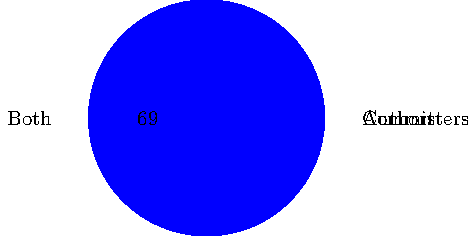
\includegraphics[height=150pt]{img/django-wiki}
    \caption{Responsibility in django-wiki}
  \end{figure}
  \vfill
\end{frame}
\begin{frame}
  \framecount{Results}
  \begin{figure}
    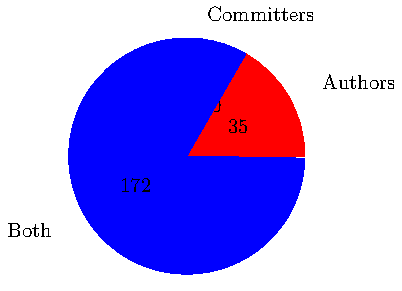
\includegraphics[height=150pt]{img/django-oscar}
    \caption{Responsibility in django-oscar}
  \end{figure}
  \vfill
\end{frame}
\begin{frame}
  \framecount{Results}
  \begin{figure}
    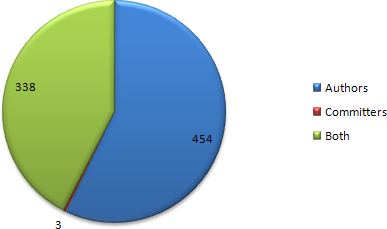
\includegraphics[height=150pt]{img/elasticsearch}
    \caption{Responsibility in elasticsearch}
  \end{figure}
  \vfill
\end{frame}

\begin{frame}
  \framecount{Results}
  \begin{figure}
    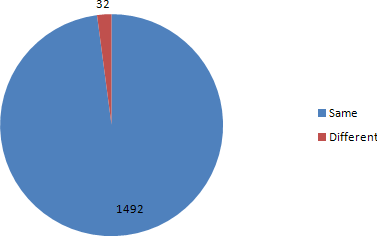
\includegraphics[height=150pt]{img/django-wiki-commits}
    \caption{Commits in django-wiki}
  \end{figure}
  \vfill
\end{frame}
\begin{frame}
  \framecount{Results}
  \begin{figure}
    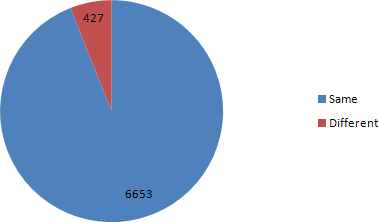
\includegraphics[height=150pt]{img/django-oscar-commits}
    \caption{Commits in django-oscar}
  \end{figure}
  \vfill
\end{frame}
\begin{frame}
  \framecount{Results}
  \begin{figure}
    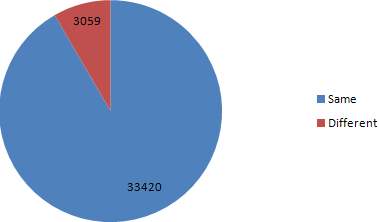
\includegraphics[height=150pt]{img/elasticsearch-commits}
    \caption{Commits in elasticsearch}
  \end{figure}
  \vfill
\end{frame}


\nextframe
\begin{frame}
    \framecount{Usage}
    \begin{itemize}
        \gitem Clone \url{https://github.com/turbopope/idman}
        \gitem Install \texttt{networkx} Python package
        \gitem Run \texttt{idman path/to/repo}
        \gitem Get Commits With Identities
    \end{itemize}
    \vfill
\end{frame}


\begin{comment}
How many developers?
How many commiters?
What is the distribution of commit counts for committers versus authors?
The team actually addresses these questions for our ``projects of interest''.
\end{comment}


%%%%%%%%%%%%%%%%%%%%%%%%%%%%%%%%%%%%%%%%%%%%%%%%%


\nextframe
\begin{frame}
    \vfill
    \begin{center}
        {\Huge Thank You All For Listening}\\
    \end{center}
\end{frame}

\end{document}
